\section{The incidence template and the nested tables}\label{sec:model}
We begin with the fixed finite combinatorics. All randomness will be in the labels, not in the template.

\subsection{Points, lines, and fans}
\begin{definition}[The incidence template]\label{def:template}
Identify the points of the projective plane over $\F_2$ with the seven nonzero vectors of $\F_2^3$. A line consists of the three nonzero vectors in a two-dimensional subspace. Fix
\[
 A=e_1,\qquad B=e_2,\qquad C=e_3,\qquad D=e_1+e_2+e_3.
\]
No three of these four points are collinear. For distinct points $i,j$, write $ij$ for their line.

The bipartite graph $\Gamma$ has a vertex $X_i$ for every point, an additional vertex $Y_i$ for $i\in\{A,B,C,D\}$, and a vertex for every line. Both representatives over a point are joined to each incident line, with one exception: the edge $Y_D$--$CD$ is omitted. The edge
\[
 e_0=X_D\text{--}CD
\]
is called the \emph{loose edge}. Every other edge belongs to the \emph{fan} $F_i$ at its point $i$. At $D$, the fan uses only the two lines other than $CD$, so $CD$ is not a vertex of $F_D$.
\end{definition}

Each $F_i$ is connected. At $A,B,C$ it is $K_{2,3}$, at $D$ it is $K_{2,2}$, and at each of the other three points it is a three-edge star. Let $g=7$ and $k_i=|E(F_i)|$. Thus
\begin{equation}\label{eq:model-counts}
 (k_i)_i=(6,6,6,4,3,3,3),\qquad
 \sum_i k_i=31,\qquad |E(\Gamma)|=32.
\end{equation}
The graph has $18$ vertices. Its cycle rank is $15$; the sum of the
cycle ranks of the fans is $7$. We will first impose the cycles within
the fans, then use a smaller graph of cycle rank $8$ to impose the
remaining core relations. The cone construction below makes this
decomposition explicit.

Figures~\ref{fig:fano-template} and~\ref{fig:fans} show the incidence
pattern and the exceptional fan.

\begin{figure}[htbp]
\centering
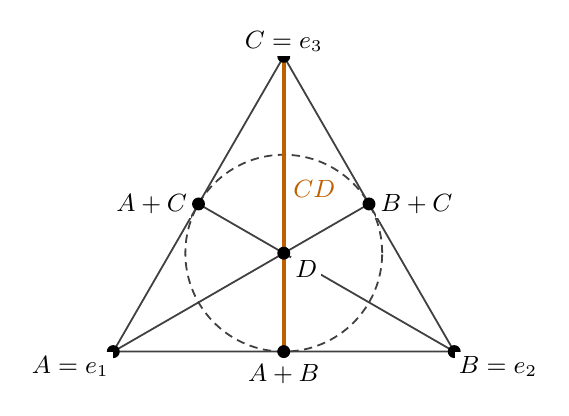
\begin{tikzpicture}[x=1.25cm,y=1.25cm,
  fano edge/.style={draw=black!75,line width=.65pt},
  fano point/.style={circle,fill=black,inner sep=1.65pt},
  fano label/.style={font=\small,fill=white,inner sep=1.5pt}]
  \coordinate (A) at ({-sqrt(3)},-1);
  \coordinate (B) at ({sqrt(3)},-1);
  \coordinate (C) at (0,2);
  \coordinate (D) at (0,0);
  \coordinate (AB) at (0,-1);
  \coordinate (AC) at ({-sqrt(3)/2},.5);
  \coordinate (BC) at ({sqrt(3)/2},.5);
  \draw[fano edge] (A)--(B)--(C)--cycle;
  \draw[fano edge] (A)--(BC) (B)--(AC);
  \draw[fano edge,densely dashed] (D) circle[radius=1];
  \draw[draw=orange!75!black,line width=1.35pt] (C)--(AB);
  \foreach \P in {A,B,C,D,AB,AC,BC}
    \node[fano point] at (\P) {};
  \node[fano label,anchor=north east] at (A) {$A=e_1$};
  \node[fano label,anchor=north west] at (B) {$B=e_2$};
  \node[fano label,anchor=south] at (C) {$C=e_3$};
  \node[fano label,anchor=north west] at (.07,-.03) {$D$};
  \node[fano label,anchor=north] at (0,-1.08) {$A+B$};
  \node[fano label,anchor=east] at ({-sqrt(3)/2-.07},.5) {$A+C$};
  \node[fano label,anchor=west] at ({sqrt(3)/2+.07},.5) {$B+C$};
  \node[fano label,anchor=west,text=orange!75!black] at (.05,.65) {$CD$};
\end{tikzpicture}
\caption{The seven points and seven lines of the Fano plane.  The three sides,
three medians, and dashed circle each represent one projective line; only
marked dots represent projective points.  The
points $A,B,C,D=A+B+C$ form a quadrangle: no three are collinear.  The thick median
is the line $CD=\{C,D,A+B\}$, at which the incidence graph is modified.}
\label{fig:fano-template}
\end{figure}

\begin{figure}[htbp]
\centering
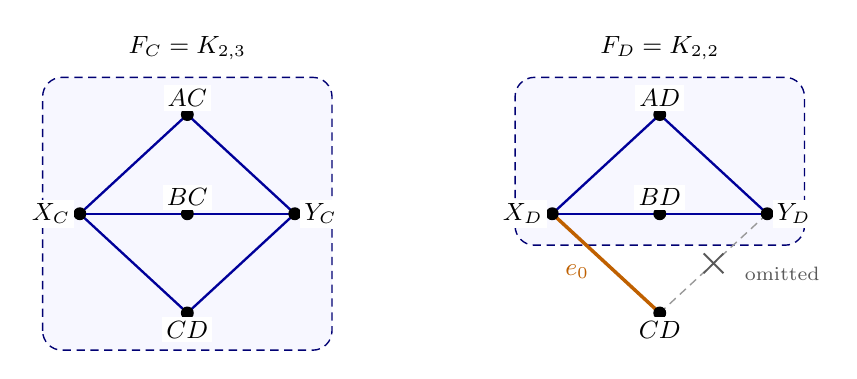
\begin{tikzpicture}[x=1.05cm,y=1.05cm,
  fan edge/.style={draw=blue!60!black,line width=.85pt},
  fan vertex/.style={circle,fill=black,inner sep=1.65pt},
  fan label/.style={font=\small,fill=white,inner sep=1.5pt},
  fan region/.style={rounded corners=7pt,draw=blue!45!black,
    densely dashed,fill=blue!3,line width=.5pt}]
  \begin{scope}[xshift=-3cm]
    \draw[fan region] (-1.75,-1.65) rectangle (1.75,1.65);
    \node[font=\small] at (0,2) {$F_C=K_{2,3}$};
    \coordinate (XC) at (-1.3,0);
    \coordinate (YC) at (1.3,0);
    \coordinate (Cac) at (0,1.2);
    \coordinate (Cbc) at (0,0);
    \coordinate (Ccd) at (0,-1.2);
    \foreach \L in {Cac,Cbc,Ccd}
      \draw[fan edge] (XC)--(\L)--(YC);
    \foreach \P in {XC,YC,Cac,Cbc,Ccd}
      \node[fan vertex] at (\P) {};
    \node[fan label,anchor=east] at (-1.36,0) {$X_C$};
    \node[fan label,anchor=west] at (1.36,0) {$Y_C$};
    \node[fan label,anchor=south] at (0,1.24) {$AC$};
    \node[fan label,anchor=south] at (0,.04) {$BC$};
    \node[fan label,anchor=north] at (0,-1.24) {$CD$};
  \end{scope}
  \begin{scope}[xshift=3cm]
    \draw[fan region] (-1.75,-.38) rectangle (1.75,1.65);
    \node[font=\small] at (0,2) {$F_D=K_{2,2}$};
    \coordinate (XD) at (-1.3,0);
    \coordinate (YD) at (1.3,0);
    \coordinate (Dad) at (0,1.2);
    \coordinate (Dbd) at (0,0);
    \coordinate (Dcd) at (0,-1.2);
    \foreach \L in {Dad,Dbd}
      \draw[fan edge] (XD)--(\L)--(YD);
    \draw[draw=orange!75!black,line width=1.25pt] (XD)--(Dcd);
    \draw[draw=black!40,densely dashed,line width=.5pt] (YD)--(Dcd);
    \draw[draw=black!65,line width=.7pt] (.53,-.48)--(.77,-.72)
                                              (.53,-.72)--(.77,-.48);
    \foreach \P in {XD,YD,Dad,Dbd,Dcd}
      \node[fan vertex] at (\P) {};
    \node[fan label,anchor=east] at (-1.36,0) {$X_D$};
    \node[fan label,anchor=west] at (1.36,0) {$Y_D$};
    \node[fan label,anchor=south] at (0,1.24) {$AD$};
    \node[fan label,anchor=south] at (0,.04) {$BD$};
    \node[fan label,anchor=north] at (0,-1.24) {$CD$};
    \node[fan label,text=orange!75!black,anchor=east] at (-.8,-.7) {$e_0$};
    \node[font=\scriptsize,anchor=west,text=black!65] at (.91,-.73) {omitted};
  \end{scope}
\end{tikzpicture}
\caption{A full fan and the exceptional fan.  The blue edges and their
endpoints form the indicated fans.  The loose edge
$e_0=X_D\text{--}CD$ belongs to $\Gamma$ but not to $F_D$; the crossed dashed
segment $Y_D\text{--}CD$ is absent from $\Gamma$.  In particular, $CD$ is
not a vertex of $F_D$.  The two occurrences of $CD$ denote the same line
vertex of $\Gamma$.}
\label{fig:fans}
\end{figure}


Choose an orientation for each edge once and for all. A \emph{field} is an edge position in a template or a position in a polygon word. An assignment gives one signed letter to each field. A walk reads that letter in the specified orientation and its inverse in the other orientation. The fields are bookkeeping coordinates; they all take values in the same alphabet.

A \emph{core hexagon} is the six-cycle obtained from three noncollinear points, the three lines joining them, and one representative over each point for which all six incidences are present. In particular, the all-$X$ choice is always permitted. Any three successive edges of a core hexagon contain at most two fields from each fan; the loose field, if present, belongs to no fan.

\FloatBarrier
\subsection{The independent tables}
For $n\ge1$, let
\[
 S_n=\{a_1,a_1^{-1},\ldots,a_n,a_n^{-1}\},\qquad N=2n.
\]
These are formal signed letters; assignments are not required to use distinct letters or to produce freely reduced words. Let
\begin{equation}\label{eq:model-parameters}
 f=2-\alpha,\qquad p=3-\beta,\qquad
 0<\alpha,\delta<1,\qquad 7\alpha<\beta<1.
\end{equation}
Additional smallness requirements will be imposed when we choose finitely many sampling tests.

\begin{definition}[The tables]\label{def:tables}
Use the following mutually independent Bernoulli arrays.
\begin{enumerate}[label=\textup{(\roman*)}]
\item For each point $i$, an array indexed by $S_n^{E(F_i)}$ includes every tuple with probability $N^{f-k_i}$. An included tuple, together with its type $i$, is a \emph{fan occurrence} $b$.
\item An array indexed by $S_n^{E(\Gamma)}$ marks every full core tuple with probability $N^{p-gf-1}$. A \emph{top occurrence} $a$ is a marked tuple whose restriction to every $F_i$ is an included fan occurrence. We write $a\to b$ when $b$ is the fan in one of the seven slots of $a$.
\item For each unoriented nonbacktracking two-edge path $\tau$ in $\Gamma$, choose one order and direction. Give $\tau$ a separate four-field array: its first two coordinates are the two core fields on $\tau$, and its last two are new coordinates. Include each row with probability $N^{-2-\delta}$. Its relator reads $\tau$, with the required orientation signs, followed by the two new letters around a closing path.
\item A separate six-field array includes each word in $S_n^6$ with probability $N^{-3-\delta}$. Its word is a relator.
\end{enumerate}
All included rows in \textup{(iii)} and \textup{(iv)} are imposed, not only rows matching some top occurrence. We call them \emph{decorations}; their lengths are $2h$, with $h\in\{2,3\}$.
\end{definition}

There is no ambiguity from opposite path directions: reversing one chosen convention simply inverts or reorders the corresponding coordinates, preserving the Bernoulli law. There are $90$ tables in Definition~\ref{def:tables}\textup{(iii)}. Indeed, the eleven point-representative vertices contribute $10\binom32+\binom22=31$ two-edge paths; the line degrees are $5,5,4,5,5,5,3$, contributing $59$ more.

The exponents in Definition~\ref{def:tables} are negative. In particular,
\[
 p-gf-1=-12-(\beta-7\alpha)<0.
\]
Each is therefore a valid probability. Distinct numerical tuples of a fixed table are independent. Top \emph{occurrences} are correlated because they may share fan slots; top \emph{marks} remain independent.

The expected counts explain the normalization of these probabilities.
For each fan type there are $N^{k_i}$ candidate tuples, so the expected
number of included fans is $N^f$. A fixed core tuple requires its mark
and seven independent fan entries. Since the fans contain $31$ fields
in total, the expected number of top occurrences is
\[
 N^{32}\,N^{p-7f-1}\prod_i N^{f-k_i}=N^p.
\]
Each square table has expected size $N^{2-\delta}$, and the six-letter
table has expected size $N^{3-\delta}$. Thus the expected exponents
are just below $2$ for fans and squares, and just below $3$ for tops
and hexagons. Section~\ref{sec:diagrams} explains how these deficits,
together with $\beta>7\alpha$, leave a positive margin in the diagram
estimates. The correlation between top occurrences is the
reason that their shared fan costs must be counted only once.

\subsection{The group and its two-complex}
The letter presentation has the generators $a_1,\ldots,a_n$. For each included fan and each top occurrence, impose the labels of all closed walks in its graph. Impose also the decoration words. This is a finite presentation: in each connected graph a fixed spanning tree supplies a finite basis of closed walks that suffices.

For the diagram arguments we use a specific finite two-dimensional CW complex $P$. Start with the letter bouquet, with vertex $o$. For each fan occurrence $b$ of type $i$, attach the cone on $F_i$ along its labelled map to the bouquet. The cone apex is a new vertex, also denoted $b$. For each vertex $v$ of $F_i$, its radial edge $r_{b,v}$ joins $b$ to the image $o$ of $v$. Every fan edge gives one triangle with one letter side and two radial sides. Different radial edges can have the same endpoints; they retain their distinct labels $v$.

The fan cones already fill all fan cycles. To impose the remaining
relations of a top occurrence $a$, take the ordinary Fano incidence
graph and subdivide the edge $D$--$CD$ once. Call the resulting graph
$B$. It has $15$ vertices and $22$ edges, hence cycle rank $8$,
matching the difference $15-7$ computed above. Map a point vertex $i$ to the apex
of the fan in slot $i$ of $a$, and map all line vertices and the
subdivision vertex to $o$. An ordinary incidence at $i$ maps to the
radial edge indexed by its line. The subdivided exceptional incidence maps to
\[
 r_{b_D,X_D}\quad\text{followed by the loose letter edge,}
\]
with the orientation giving the path from $X_D$ to $CD$. Attach the cone on this mapped graph, with its own new apex. We call its radial triangles \emph{top triangles}. Finally attach every decoration polygon. All these attachments are finite, and $P$ has dimension two.

\begin{lemma}[Presentation equivalence]\label{lem:model-presentation}
The complex $P$ has the fundamental group of the letter presentation above. In particular, it has a quotient isomorphic to $C_2$.
\end{lemma}
\begin{proof}
For a connected graph $H$ and a map $H\to X$ into a connected complex, attaching its cone changes $\pi_1X$ by the normal closure of the image of $\pi_1H$. It introduces no extra generator. This follows from van Kampen, or by choosing a spanning tree of $H$ and eliminating all but one of the new radial edges successively. The statement does not require distinct graph vertices to have distinct images.

It remains to check that the top macro graph imposes the required core relations after the fan relations. Each fan triangle replaces a fan edge by the two radial edges from its endpoints to the fan apex. A path in a fan can therefore be replaced, relative its endpoints, by the radial path through that apex. Apply these replacements to a closed core walk. Excursions through $X_i$ or $Y_i$ then cancel, leaving a closed walk in the mapped macro graph. At $D$, the only unreplaced edge is the loose edge; together with $r_{b_D,X_D}$ it gives exactly the exceptional subdivided incidence. Conversely, every macro turn can be replaced by a path in its connected fan. The two sets of relations have the same normal closure modulo the fan relations. This proves the presentation assertion.

The graph $\Gamma$, and each fan, is bipartite, so every closed-walk word has even length. The decorations have lengths four and six. Sending each original generator to the nonidentity element of $C_2$ respects all the defining relations and is surjective.
\end{proof}

\begin{remark}\label{rem:model-finite}
The cone description records occurrences, not just relator words. If the same fan occurs in several tops, its cone is attached only once. A top occurrence has its own cone, and a decoration occurrence has its own disk. These distinctions are essential in the multiplicity count of Section~\ref{sec:diagrams}.
\end{remark}

\subsection{The master pattern and admissible tests}
Define the finite \emph{master pattern} $\mathcal M$ by taking one top occurrence with its seven fan slots and, for each of the $90$ two-edge paths, one matching row of its square table. The two core coordinates of that row are identified with their core fields; its two closing coordinates are new. The separate six-letter array is not part of $\mathcal M$.

A \emph{match} is an assignment to the fields of $\mathcal M$ for which every required table entry is present, including the top mark. We denote the set of matches by $\Omega_n$. When it is nonempty, it carries its uniform probability measure. Its $32+2\cdot90$ fields include the shared core fields only once.

\begin{definition}[Admissible fields]\label{def:admissible}
A set of fields is \emph{admissible} if it is either
\begin{enumerate}[label=\textup{(\roman*)}]
\item a set of at most three distinct core fields containing at most two fields of each fan, or
\item a set of at most two fields of a single square decoration in $\mathcal M$.
\end{enumerate}
The loose core field does not count against any fan quota.
\end{definition}

The first case includes all three-edge half-paths of core hexagons. It also includes two $F_C$ fields together with the loose field, the combination that will produce the decisive midpoint identity. The second case includes every two-edge half-path in a decoration square.

Every match has a labelled realization of the core graph and the closing paths of its square decorations in the group: fix an anchor, and label a vertex by the word read along any path from the anchor. All closed-path labels are trivial by Lemma~\ref{lem:model-presentation} and the square relators. Consequently this group-valued vertex assignment is independent of the chosen path. For any action and basepoint, it gives a corresponding configuration of orbit points.
